\chapter{Review}

The last chapter mainly focuses on the box model's evalution to the requirements specified during the planning phase, shortcomings and how these could potentially be overcome and finally, opportunities of further development and additional ideas.

\section{Usage}

During usage, controlling the model box's components via the user interface is quite impressive, as when components are toggled or values are altered from a laptop or smartphone, the changes made propagate really fast to the model, in a few seconds at most. Besides control, monitoring of the implemented sensors is also reliable, as when influenced externally eg. less or more heat, light are applied to them, a change can be seen in the readings of sensors. These values, along with other metrics, actions taken by the user are continuously logged and this history can be reviewed later, or even be plotted to a graph in case of quantifiable amounts, between certain time ranges.

\begin{figure}[!ht]
    \centering
    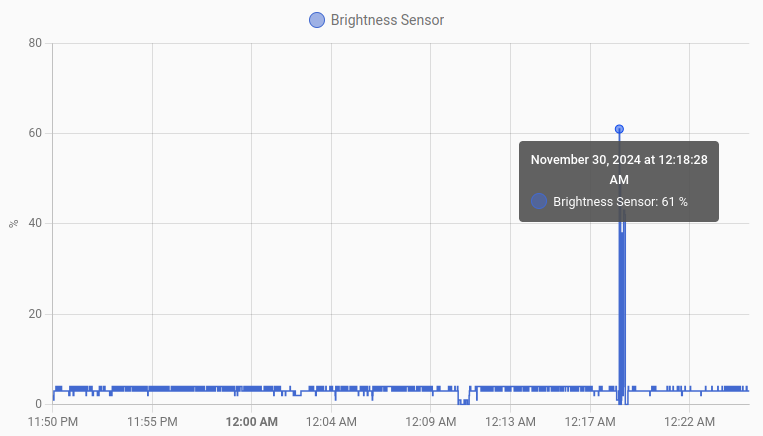
\includegraphics[width=110mm, keepaspectratio]{figures/homeassistant_graph_history.png}
    \caption{Home Assistant history graph for the LDR (in a dark environment, the outstanding values show when a flashlight was shined upon it)}
    \label{fig:HAgraphHistory}
  \end{figure}

The use cases of the model include the most important aspects of a typical smart home environment: monitoring of temperature and light levels, control of basic utilities in the form of heating and cooling, and lastly, a "smartified" rolling shutter (that would be actuated by hand in a conventional home).

\section{Critical analysis, shortcomings}

The experience of using the model box and its user interface is really similar to what a deployed home environment would be, therefore an adequate way to simulate a real smart home system with certain limitations. The model features a full-fledged smart home software platform, which is used in many installations worldwide. % todo source based on github stars, or that it is one of the most popular open source projects
The number of "devices" (according to Home Assistant's terminology) is less, than in a usual real environment with more heterogeneous devices, but the number components connected to it makes it comparable to that of a basic installation.
There are aspects however, that are usually part of a typical installation, but weren't featured in the model, these are security management and energy monitoring systems (besides the solar power car charging simulation), due to the limited scope and resources of the project. They could be simulated with more components added, but it would have increased the project's cost, it is also possible that an other microcontroller would have been needed.

With the selected software platforms and devices, the user has absolute control over their smart home infrastructure and its data. With the proper knowledge, it can be changed, further developed and expanded with additional modules due to its open-source nature. In a typical installation, the smart home platform would be run on an always running computer, server or low-powered microcomputer (eg. Raspberry Pi), along with an uninterrupted power supply (UPS) to prevent data loss and quicker recovery from momentary power disruption, instead of running from a laptop, that always transported to different locations. However, the system's operation and management requires basic IT system administration knowledge, that many smart home end-users lack, therefore this solution might not be favorable for them and should utilize easier to set-up, out-of-the-box solutions, or hire a contractor, who is specialized in smart home system installations and maintenance.

A smart home platform, its network communication medium and connected devices, appliances should function realiably. If this is not the case and one or more utilities aren't available, their unavailability can cause different levels of inconvenience to the inhabitants of the house. This can range from minor sensor readings not available or updated, to lights or hot water for shower not available, to the lack of heating during winter or air conditioning during summer.

A smart home platform should also have adequate security measures, as its security is only as strong as its weakest link. The demo box uses a separated Wi-Fi network with a decent pre-shared-key (password) and encryption (WPA2), and the control server is only accessible from this Wi-Fi network or the development laptop and requires authentication with custom credentials set. It is not accessible from the Internet (it is behind Network Address Translation), but a typical environment would be set up for access, therefore security is even more important in that case. If such systems are hacked into, it can have varying negative consequences to their owners: starting from toggling and changing values of appliances, gatewaying into the home network via a compromised device to find additional vulnerabilities, to theft of data and spying in the form of video or audio means (if a camera or voice system is installed). Therefore it is crucial to ensure security, software updates should be installed regularly (and these shouldn't introduce new vulnerabilities or bugs, as it sometimes happens by some irresponsible manufacturers).

The model box's hardware doesn't suffer from vendor lock-in, as it often is with many commercial smart home solutions. The platform is modular, parts can be substituted, added and further developed thanks to its open-source nature. However, changing the software platforms can still be tedious and time-consuming, as the environments need to be set up again and customized to the specific needs of the users and exact environment, and can take between hours to days in a typical home installation.

\section{Opportunities of further development}

The model can be further developed in its current hardware form with additional software features, eg. with an automatic thermostat set to a target temperature and dashboard improvements. With additional hardware components, the currently missing subsystems (eg. security with card readers and RFID cards, energy monitoring with a power meter for electricity and its continuous logging) can be added, however this might require the utilization of a second microcontroller (which ideally should have the same microcontroller architecture), due to the limited number of remanining free pins and the features that these provide (eg. PWM, ADC, DAC) not being enough on the first.

An even larger leap for the project would be to be deployed in a real house in a more production-grade environment. The controller software should be installed on an always-on computer, server or microcomputer (eg. Raspberry Pi). It should be connected to an uninterrupted power supply (UPS) for less downtime during power outages. The devices utilized would be larger, higher power specialized appliances with a hardware platform capable for controlling electricals, communicating to the control server and firmware with integrations to the specific smart home platform, optionally changeable to an open-source variant.

Newer, more efficient IoT communication protocols and devices can be also tried out and added to the system, such as Z-Wave, Zigbee and Matter. They can achieve less power consumption, less crowding of the ISM bands (as many Wi-Fi, Bluetooth devices tend to overload the 2.4 GHz band), mesh networking to achieve better range and more compatibility between devices from different manufacturers.

Besides trying out new protocols and technologies utilizing them, there is also a need for further development of these software and hardware solutions in the field of IoT and home automation. The demand for such solutions is steadily increasing, therefore the development and operation of these solutions can be a profitable business idea, as noted in the introduction.
